\documentclass[a4paper]{article}

\usepackage[a4paper, total={18cm, 26cm}]{geometry}
\usepackage[T1]{fontenc} % needed by beramono
\usepackage{textcomp}
\usepackage[hidelinks]{hyperref}
\usepackage{float}
% beramono.sty and MnSymbol.sty come with texlive-fonts-extra in Debian
\usepackage[scaled=0.85]{beramono} % tt font supporting slshape and zero with dot
\usepackage{MnSymbol} % fancy symbols for line-breaks
\usepackage[utf8]{inputenc}
\usepackage{listingsutf8}  % code listings, comes with texlive-latex-recommended
%\usepackage{listings}
\usepackage{xcolor}
\usepackage{verbatim}
\usepackage{graphicx} % \includegraphics[width=\textwidth]{image.png}

\title{Stochastic Simulation Library}
\author{Patrick Frostholm Østergaard\\Student No.: 20195087 \\ \url{pfas19@student.aau.dk}}
\date{\today}

\begin{document}
\maketitle

This report documents my implementation of the Stochastic Simulation Library for the Selected Topics in Programming course exam at AAU 2023.

The source code for the project can also be found in my \href{https://github.com/Pattrigue/selected-topics-in-programming}{\color{blue}GitHub repository} for the course.

\section{Project Files}
% \protected\def\plusminus{\ensuremath{\pm}}
% \DeclareUnicodeCharacter{C2B1}{\plusminu\}newcommand{\plusminus}{\ensuremath{\pm}}

\lstset{
  inputencoding=utf8,
  literate={±}{\plusminus}1
}

\lstdefinestyle{bwC++}{
  language=C++,
  morekeywords={concept,consteval,constinit,constexpr,co_await,co_return,co_yield,requires},
  basicstyle=\ttfamily,
  keywordstyle=\bfseries,
  stringstyle=\slshape,
  commentstyle=\slshape,
  morecomment=[s][\bfseries\slshape]{/**}{*/},
  tabsize=4,
  showstringspaces=false,
  breaklines=true, breakatwhitespace=true,
  prebreak={\hbox{\quad$\rhookswarrow$}},
  postbreak={\hbox{$\lhookrightarrow$}},
  breakindent={-8pt}, breakautoindent=false,
  numbers=left, numberstyle=\tiny,
  frameshape={RYR}{N}{N}{YYY} %frame=tb,frameround=tttt
}

\lstdefinestyle{colorC++}{
  language=C++,
  morekeywords={concept,consteval,constinit,constexpr,co_await,co_return,co_yield,requires},
  basicstyle=\ttfamily,
  keywordstyle=\textcolor{blue},
  stringstyle=\slshape\textcolor{red!70!black},
  commentstyle=\slshape\textcolor{green!50!black},
  morecomment=[s][\bfseries\slshape\textcolor{green!50!black}]{/**}{*/},
  tabsize=4,
  showstringspaces=false,
  breaklines=true, breakatwhitespace=true,
  prebreak={\hbox{\quad\textcolor{red}{$\rhookswarrow$}}},
  postbreak={\hbox{\textcolor{red}{$\lhookrightarrow$}}},
  breakindent={-8pt}, breakautoindent=false,
  numbers=left, numberstyle=\tiny,
  frameshape={RYR}{N}{N}{YYY} %frame=tb,frameround=tttt
}

\lstdefinestyle{colorBash}{
  language=bash,
  basicstyle=\ttfamily,
  keywordstyle=\textcolor{blue},
  stringstyle=\slshape\textcolor{red!70!black},
  commentstyle=\slshape\textcolor{green!50!black},
  morecomment=[s][\bfseries\slshape\textcolor{green!50!black}]{/**}{*/},
  tabsize=4,
  showstringspaces=false,
  breaklines=true, breakatwhitespace=true,
  prebreak={\hbox{\quad\textcolor{red}{$\rhookswarrow$}}},
  postbreak={\hbox{\textcolor{red}{$\lhookrightarrow$}}},
  breakindent={-8pt}, breakautoindent=false,
  numbers=left, numberstyle=\tiny,
  frameshape={RYR}{N}{N}{YYY} %frame=tb,frameround=tttt
}

\lstdefinestyle{python}{
  language=Python,
  morekeywords={as},
  basicstyle=\ttfamily,
  keywordstyle=\color{blue},
  stringstyle=\color{red!70!black},
  commentstyle=\color{green!50!black},
  morecomment=[s][\bfseries\slshape\color{green!50!black}]{"""}{"""},
  tabsize=4,
  showstringspaces=false,
  breaklines=true,
  prebreak=\raisebox{0ex}[0ex][0ex]{\ensuremath{\hookleftarrow}},
  postbreak=\raisebox{0ex}[0ex][0ex]{\ensuremath{\hookrightarrow}},
  numbers=left,
  numberstyle=\tiny,
  frame=tb,
  frameround=tttt
}

The following two sections show the CMakeLists.txt files used to build the project as well as the source code itself.
I used CLion as my IDE on Windows 11 with the bundled toolchains.
Please see Figure \ref{fig:toolchains} for the toolchains setup.

\begin{figure}[H]
  \centering
  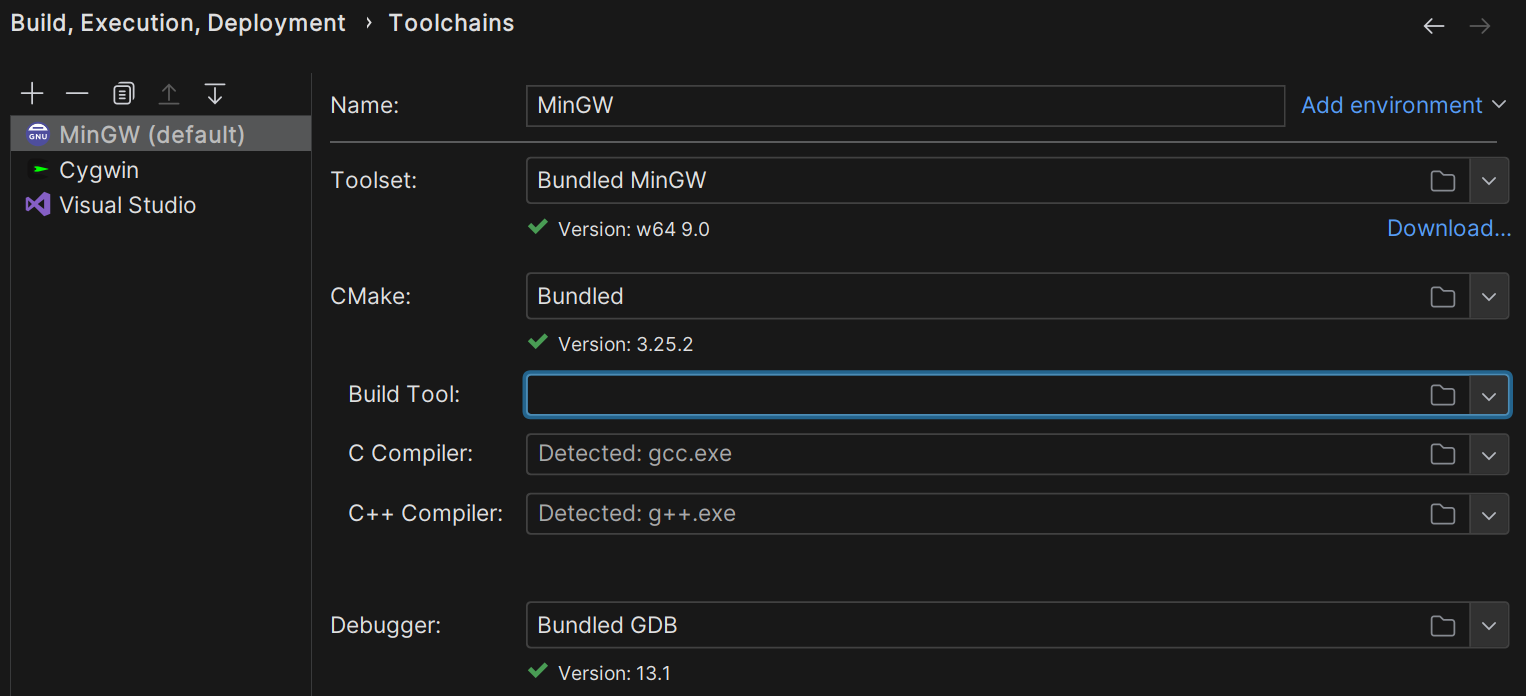
\includegraphics[width=0.8\textwidth]{toolchains.png}
  \caption{Toolchains setup in CLion.}
  \label{fig:toolchains}
\end{figure}

\begin{figure}[H]
  \centering
  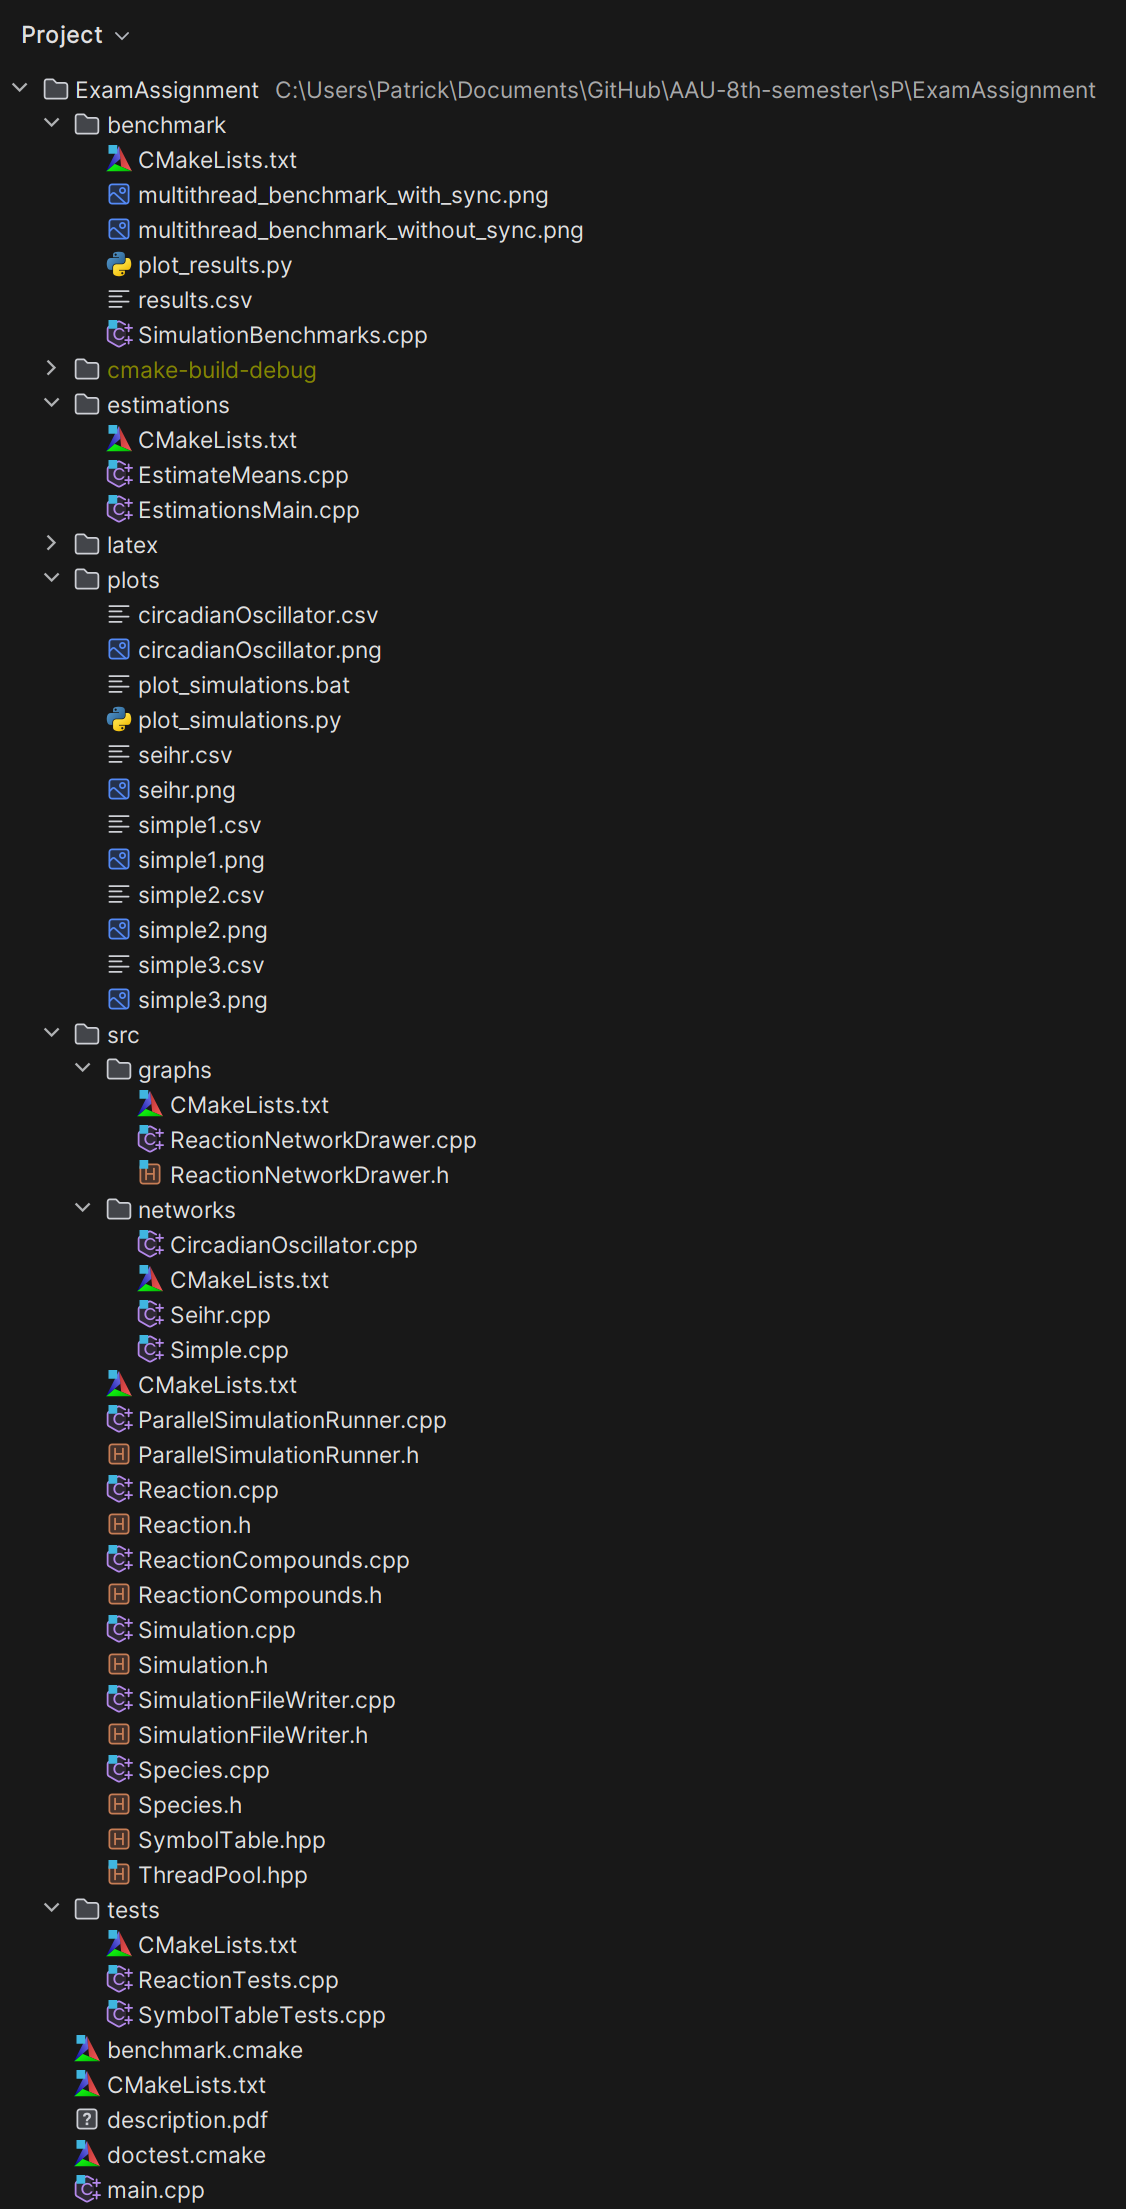
\includegraphics[width=0.675\textwidth]{project_structure.png}
  \caption{Project structure in CLion.}
  \label{fig:project_structure}
\end{figure}

In addition, Figure \ref{fig:project_structure} shows the project structure in CLion.

\subsection{CMakeLists}
The following listings show the CMakeLists.txt files used to build the project.

\lstinputlisting[style=colorBash,caption={CMakeLists.txt}]{../CMakeLists.txt}
\lstinputlisting[style=colorBash,caption={src/CMakeLists.txt}]{../src/CMakeLists.txt}
\lstinputlisting[style=colorBash,caption={src/networks/CMakeLists.txt}]{../src/networks/CMakeLists.txt}
\lstinputlisting[style=colorBash,caption={src/graphs/CMakeLists.txt}]{../src/graphs/CMakeLists.txt}
\lstinputlisting[style=colorBash,caption={estimations/CMakeLists.txt}]{../estimations/CMakeLists.txt}
\lstinputlisting[style=colorBash,caption={tests/CMakeLists.txt}]{../tests/CMakeLists.txt}
\lstinputlisting[style=colorBash,caption={benchmark/CMakeLists.txt}]{../benchmark/CMakeLists.txt}

\subsection{Source code}
The following listings show the source code for the project.
While I used the \texttt{Graphviz} C API for the graphs, I used \texttt{matplotlib} in Python for the plots, as external tools were allowed.

\lstinputlisting[style=colorC++,caption={src/Species.h}]{../src/Species.h}
\lstinputlisting[style=colorC++,caption={src/Species.cpp}]{../src/Species.cpp}

\lstinputlisting[style=colorC++,caption={src/Reaction.h}]{../src/Reaction.h}
\lstinputlisting[style=colorC++,caption={src/Reaction.cpp}]{../src/Reaction.cpp}

\lstinputlisting[style=colorC++,caption={src/ReactionCompounds.h}]{../src/ReactionCompounds.h}
\lstinputlisting[style=colorC++,caption={src/ReactionCompounds.cpp}]{../src/ReactionCompounds.cpp}

\lstinputlisting[style=colorC++,caption={src/Simulation.h}]{../src/Simulation.h}
\lstinputlisting[style=colorC++,caption={src/Simulation.cpp}]{../src/Simulation.cpp}

\lstinputlisting[style=colorC++,caption={src/ParallelSimulationRunner.h}]{../src/ParallelSimulationRunner.h}
\lstinputlisting[style=colorC++,caption={src/ParallelSimulationRunner.cpp}]{../src/ParallelSimulationRunner.cpp}

\lstinputlisting[style=colorC++,caption={src/SimulationFileWriter.h}]{../src/SimulationFileWriter.h}
\lstinputlisting[style=colorC++,caption={src/SimulationFileWriter.cpp}]{../src/SimulationFileWriter.cpp}

\lstinputlisting[style=colorC++,caption={src/SymbolTable.hpp}]{../src/SymbolTable.hpp}

\lstinputlisting[style=colorC++,caption={src/ThreadPool.hpp}]{../src/ThreadPool.hpp}

\lstinputlisting[style=colorC++,caption={src/networks/Simple.cpp}]{../src/networks/Simple.cpp}

\lstinputlisting[style=colorC++,caption={src/networks/Seihr.cpp}]{../src/networks/Seihr.cpp}

\lstinputlisting[style=colorC++,caption={src/networks/CircadianOscillator.cpp}]{../src/networks/CircadianOscillator.cpp}

\lstinputlisting[style=colorC++,caption={src/graphs/ReactionNetworkDrawer.h}]{../src/graphs/ReactionNetworkDrawer.h}
\lstinputlisting[style=colorC++,caption={src/graphs/ReactionNetworkDrawer.cpp}]{../src/graphs/ReactionNetworkDrawer.cpp}

\lstinputlisting[style=colorC++,caption={estimations/EstimateMeans.cpp}]{../estimations/EstimateMeans.cpp}
\lstinputlisting[style=colorC++,caption={EstimationsMain.cpp},label={lst:EstimationsMain.cpp}]{../estimations/EstimationsMain.cpp}

\lstinputlisting[style=colorC++,caption={tests/ReactionTests.cpp}]{../tests/ReactionTests.cpp}

\lstinputlisting[style=colorC++,caption={tests/SymbolTableTests.cpp}]{../tests/SymbolTableTests.cpp}

\lstinputlisting[style=python,caption={plots/plot\_simulations.py}]{../plots/plot_simulations.py}

\lstinputlisting[style=python,caption={benchmark/plot\_results.py}]{../benchmark/plot_results.py}

\lstinputlisting[style=colorC++,caption={benchmark/SimulationBenchmarks.cpp}]{../benchmark/SimulationBenchmarks.cpp}

\lstinputlisting[style=colorC++,caption={main.cpp}]{../main.cpp}


\section{Figures}
\subsection{Reaction Networks}
\begin{figure}[H]
    \begin{minipage}[t][6cm][t]{.18\textwidth}
        \centering
        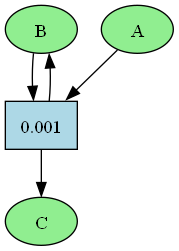
\includegraphics[width=\linewidth]{networks/simple.png}
        \caption{Reaction network for the simple model.}
        \label{fig:network_simple}
    \end{minipage}\hfill
    \begin{minipage}[t][6cm][t]{.38\textwidth}
        \centering
        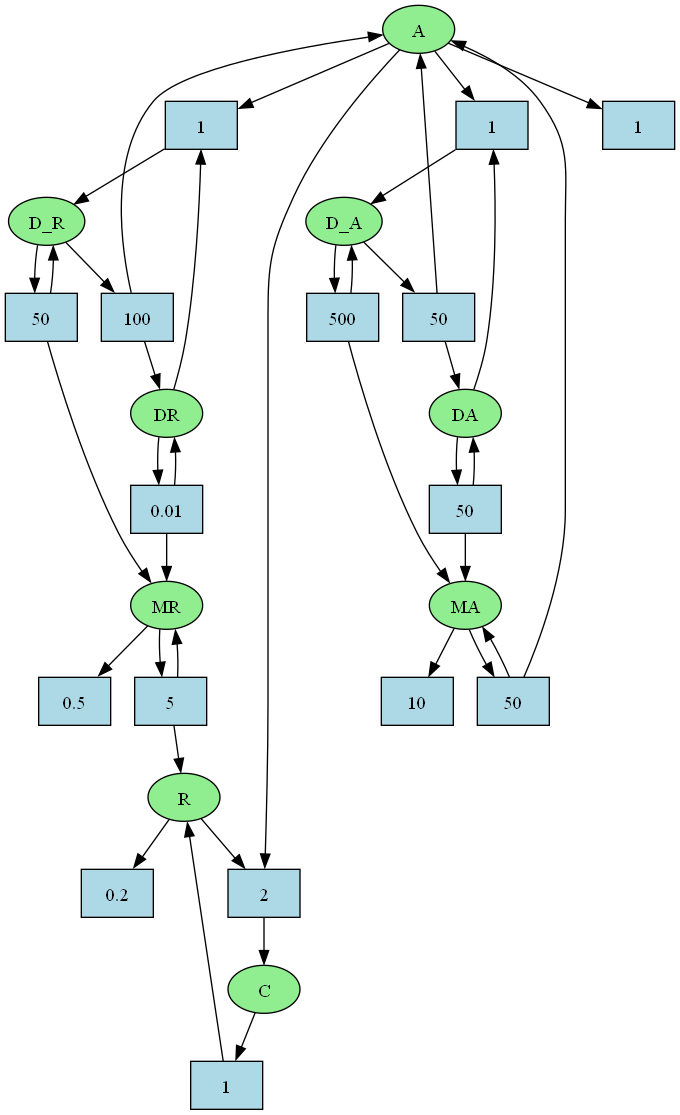
\includegraphics[width=\linewidth]{networks/circadianOscillator.png}
        \caption{Reaction network for the circadian oscillator model.}
        \label{fig:network_circadianOscillator}
    \end{minipage}\hfill
    \begin{minipage}[t][6cm][t]{.38\textwidth}
        \centering
        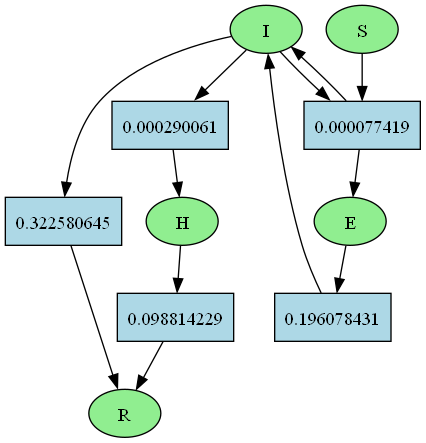
\includegraphics[width=\linewidth]{networks/seihr.png}
        \caption{Reaction network for the SEIHR model.}
        \label{fig:network_seihr}
    \end{minipage}
\end{figure}

\subsection{Plots}
\begin{figure}[H]
	\centering
	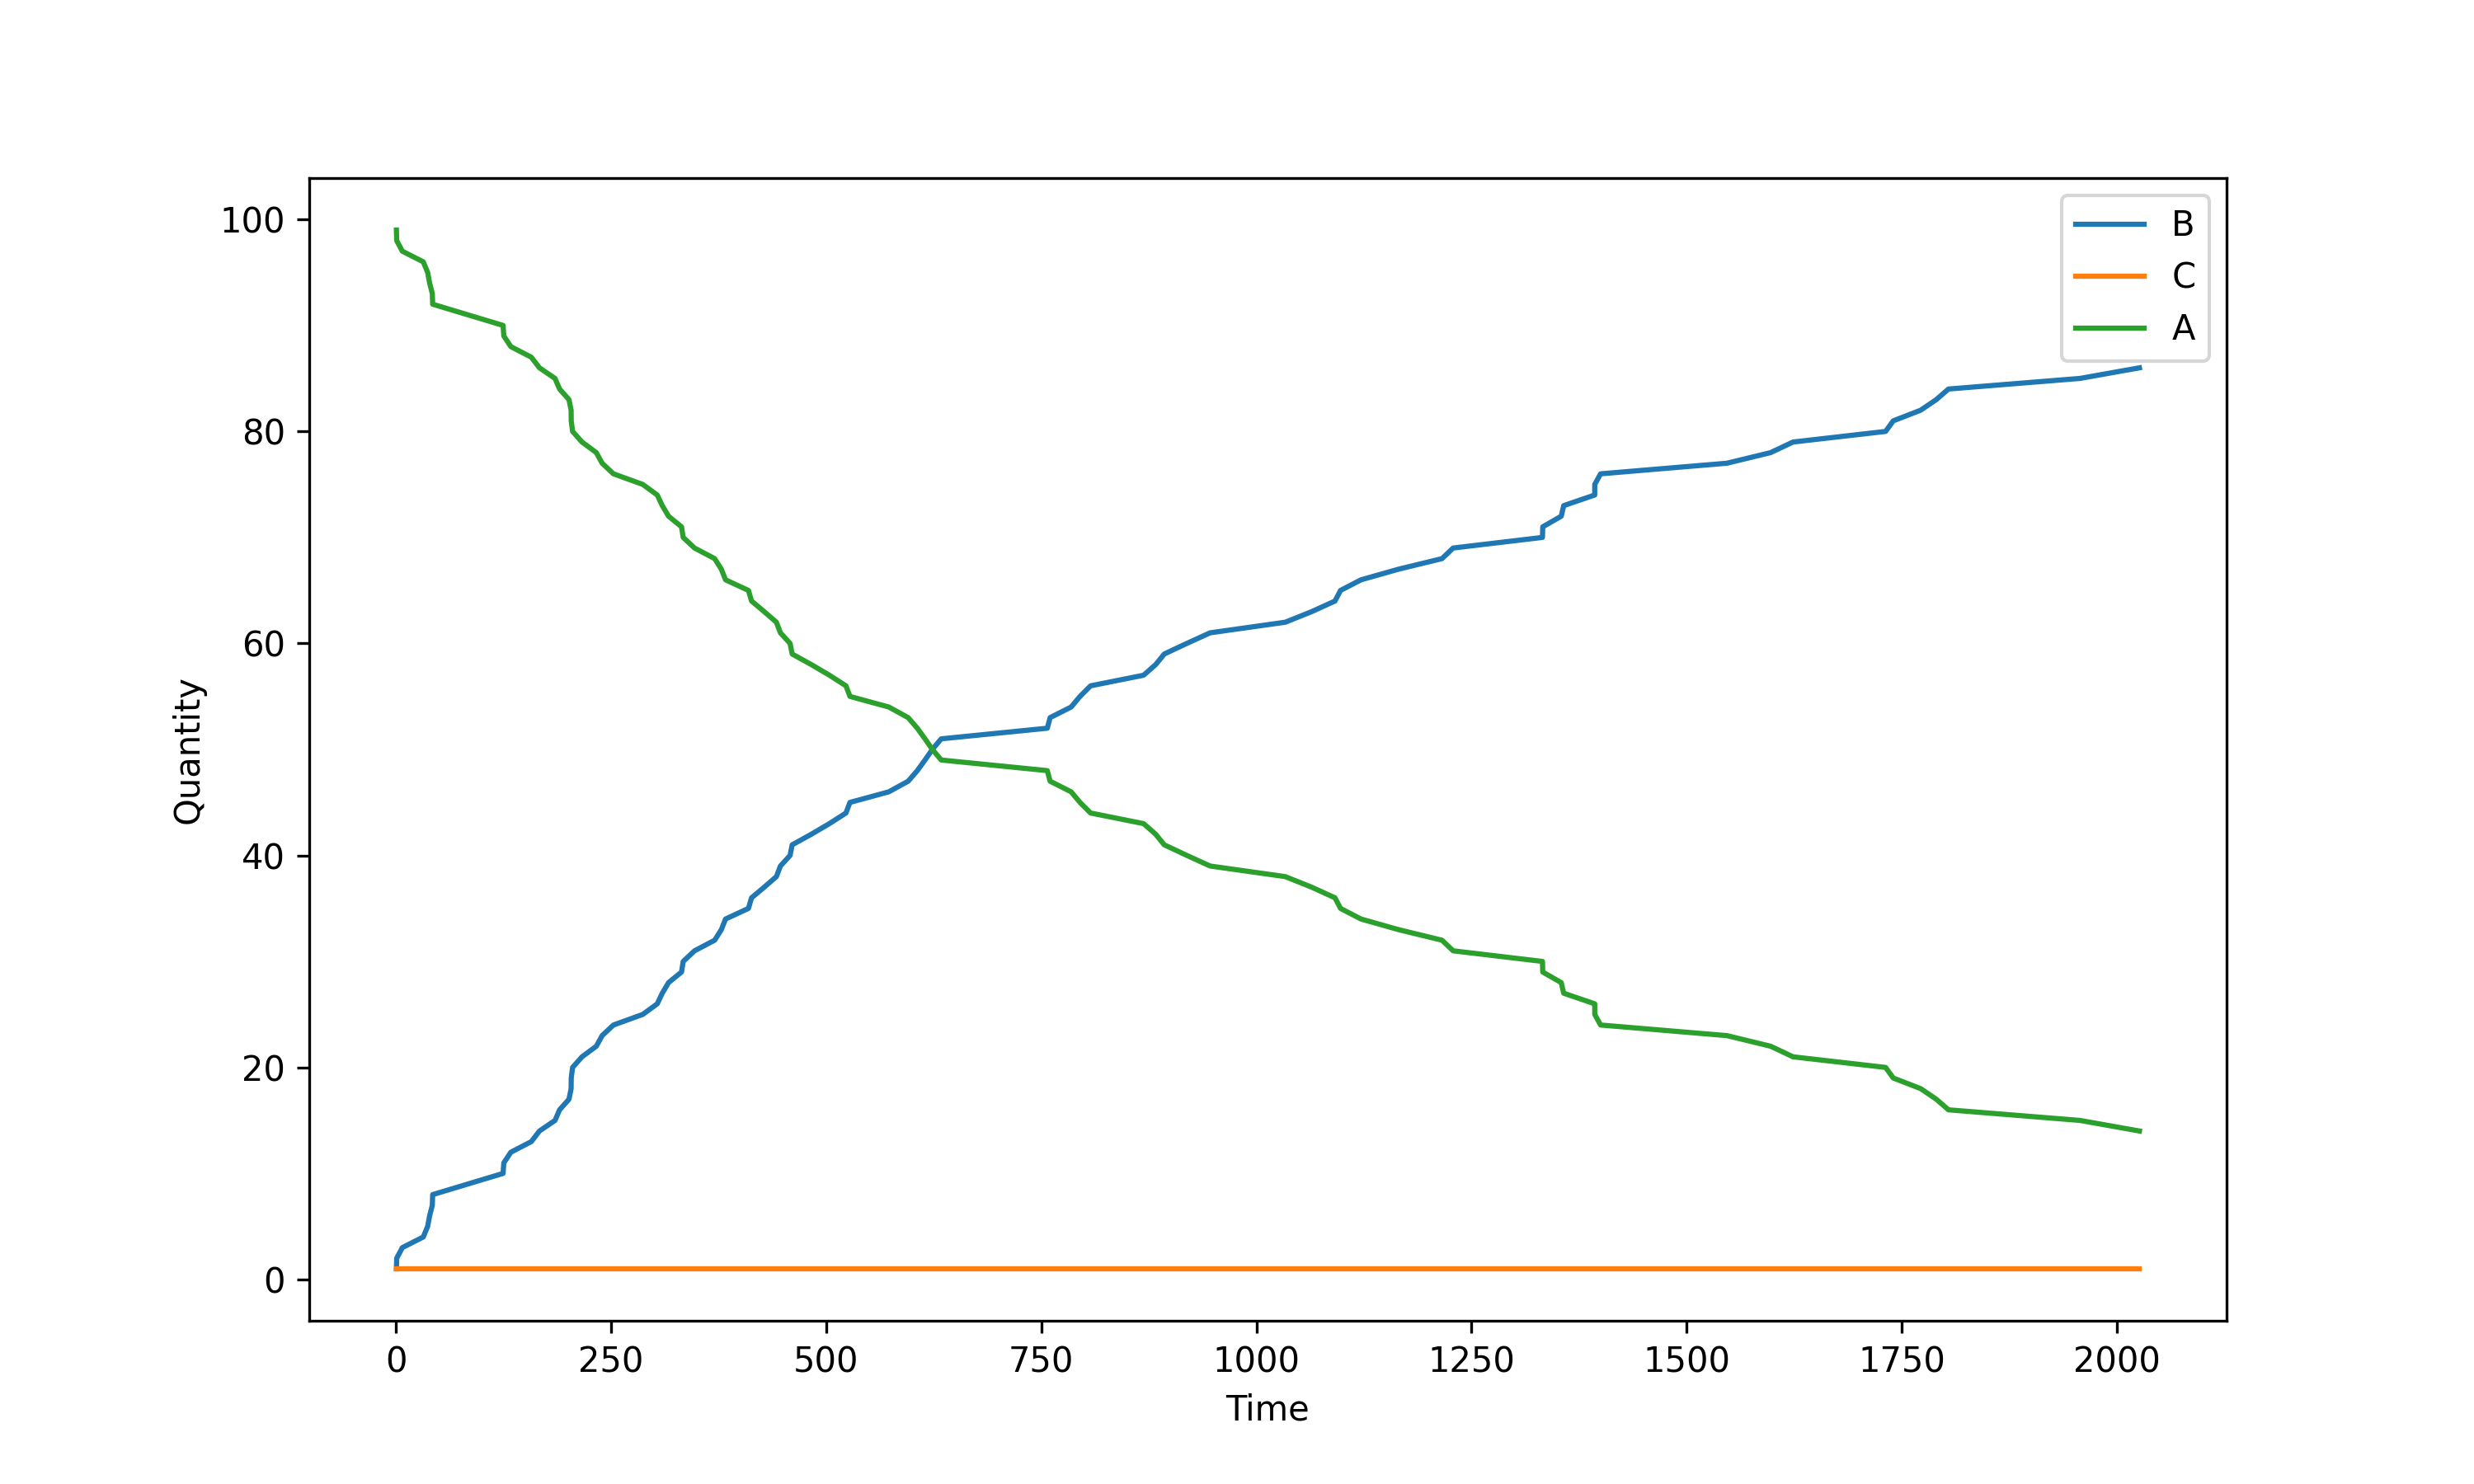
\includegraphics[width=\textwidth]{../plots/simple1}
	\caption{Plot of running the simple model simulation with A(0)=100, B(0)=0, C(0)=1.}
	\label{fig:plot_simple1}
\end{figure}

\begin{figure}[H]
	\centering
	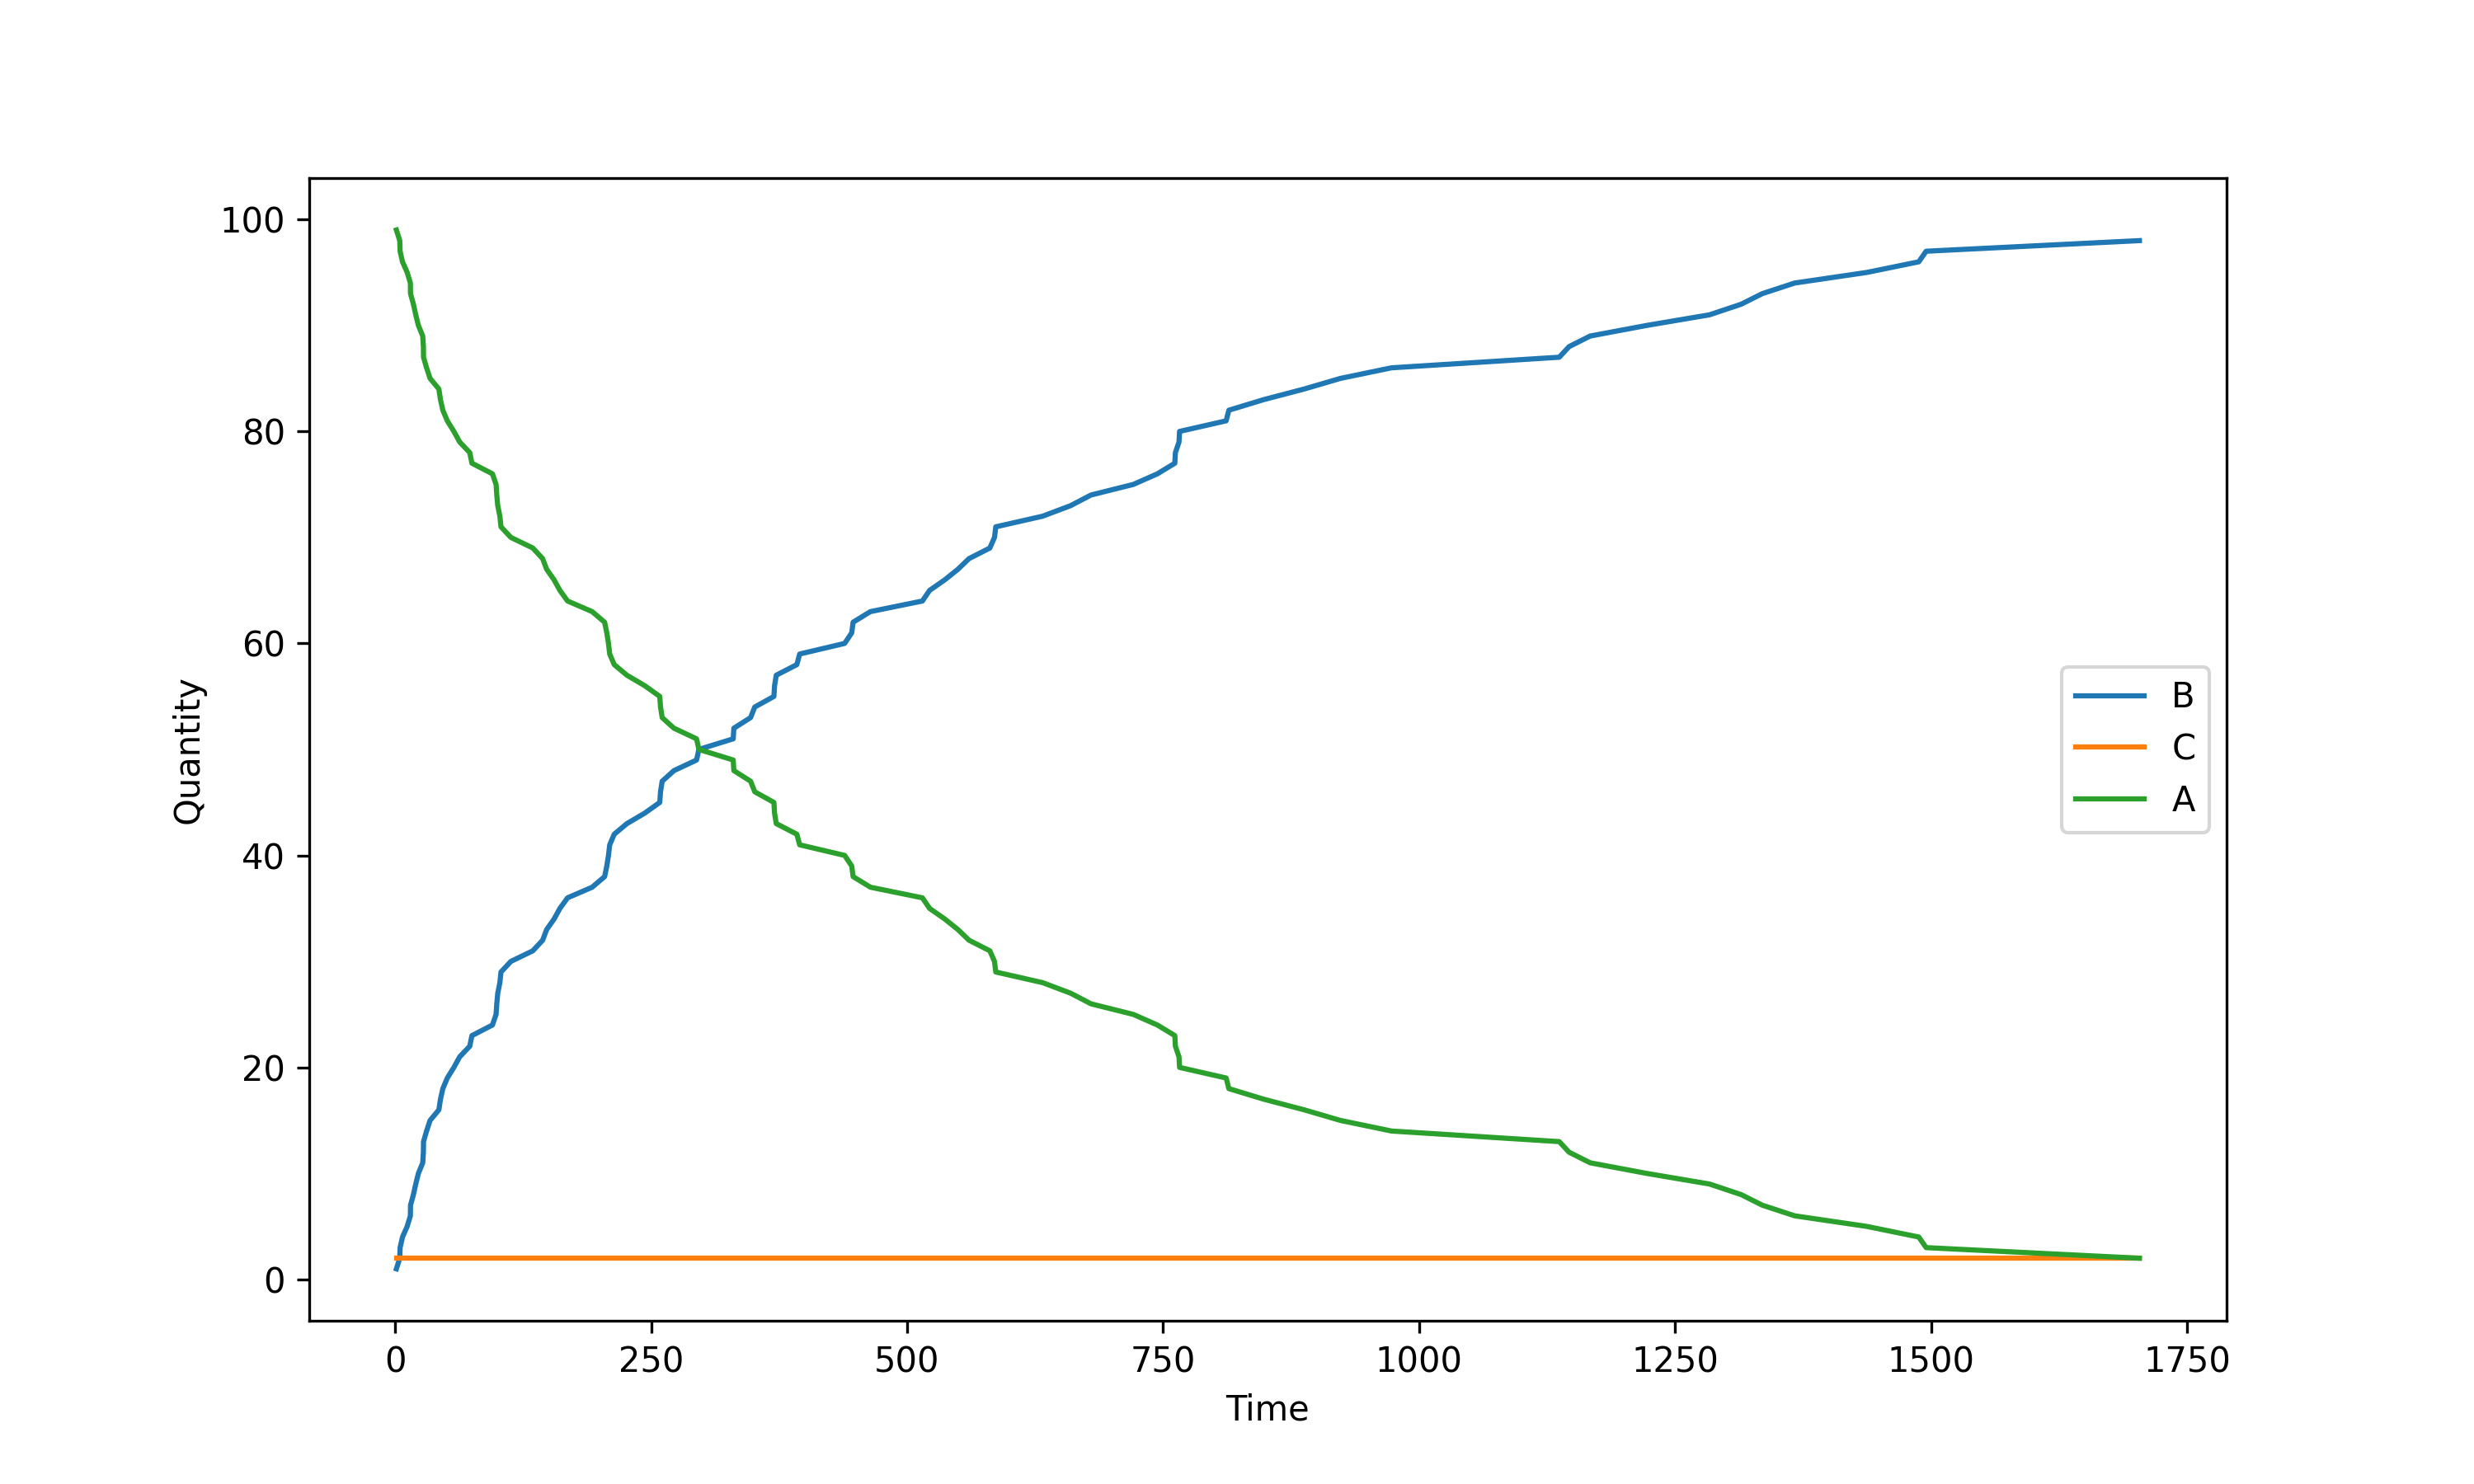
\includegraphics[width=\textwidth]{../plots/simple2}
	\caption{Plot of running the simple model simulation with A(0)=100, B(0)=0, C(0)=2.}
	\label{fig:plot_simple2}
\end{figure}

\begin{figure}[H]
	\centering
	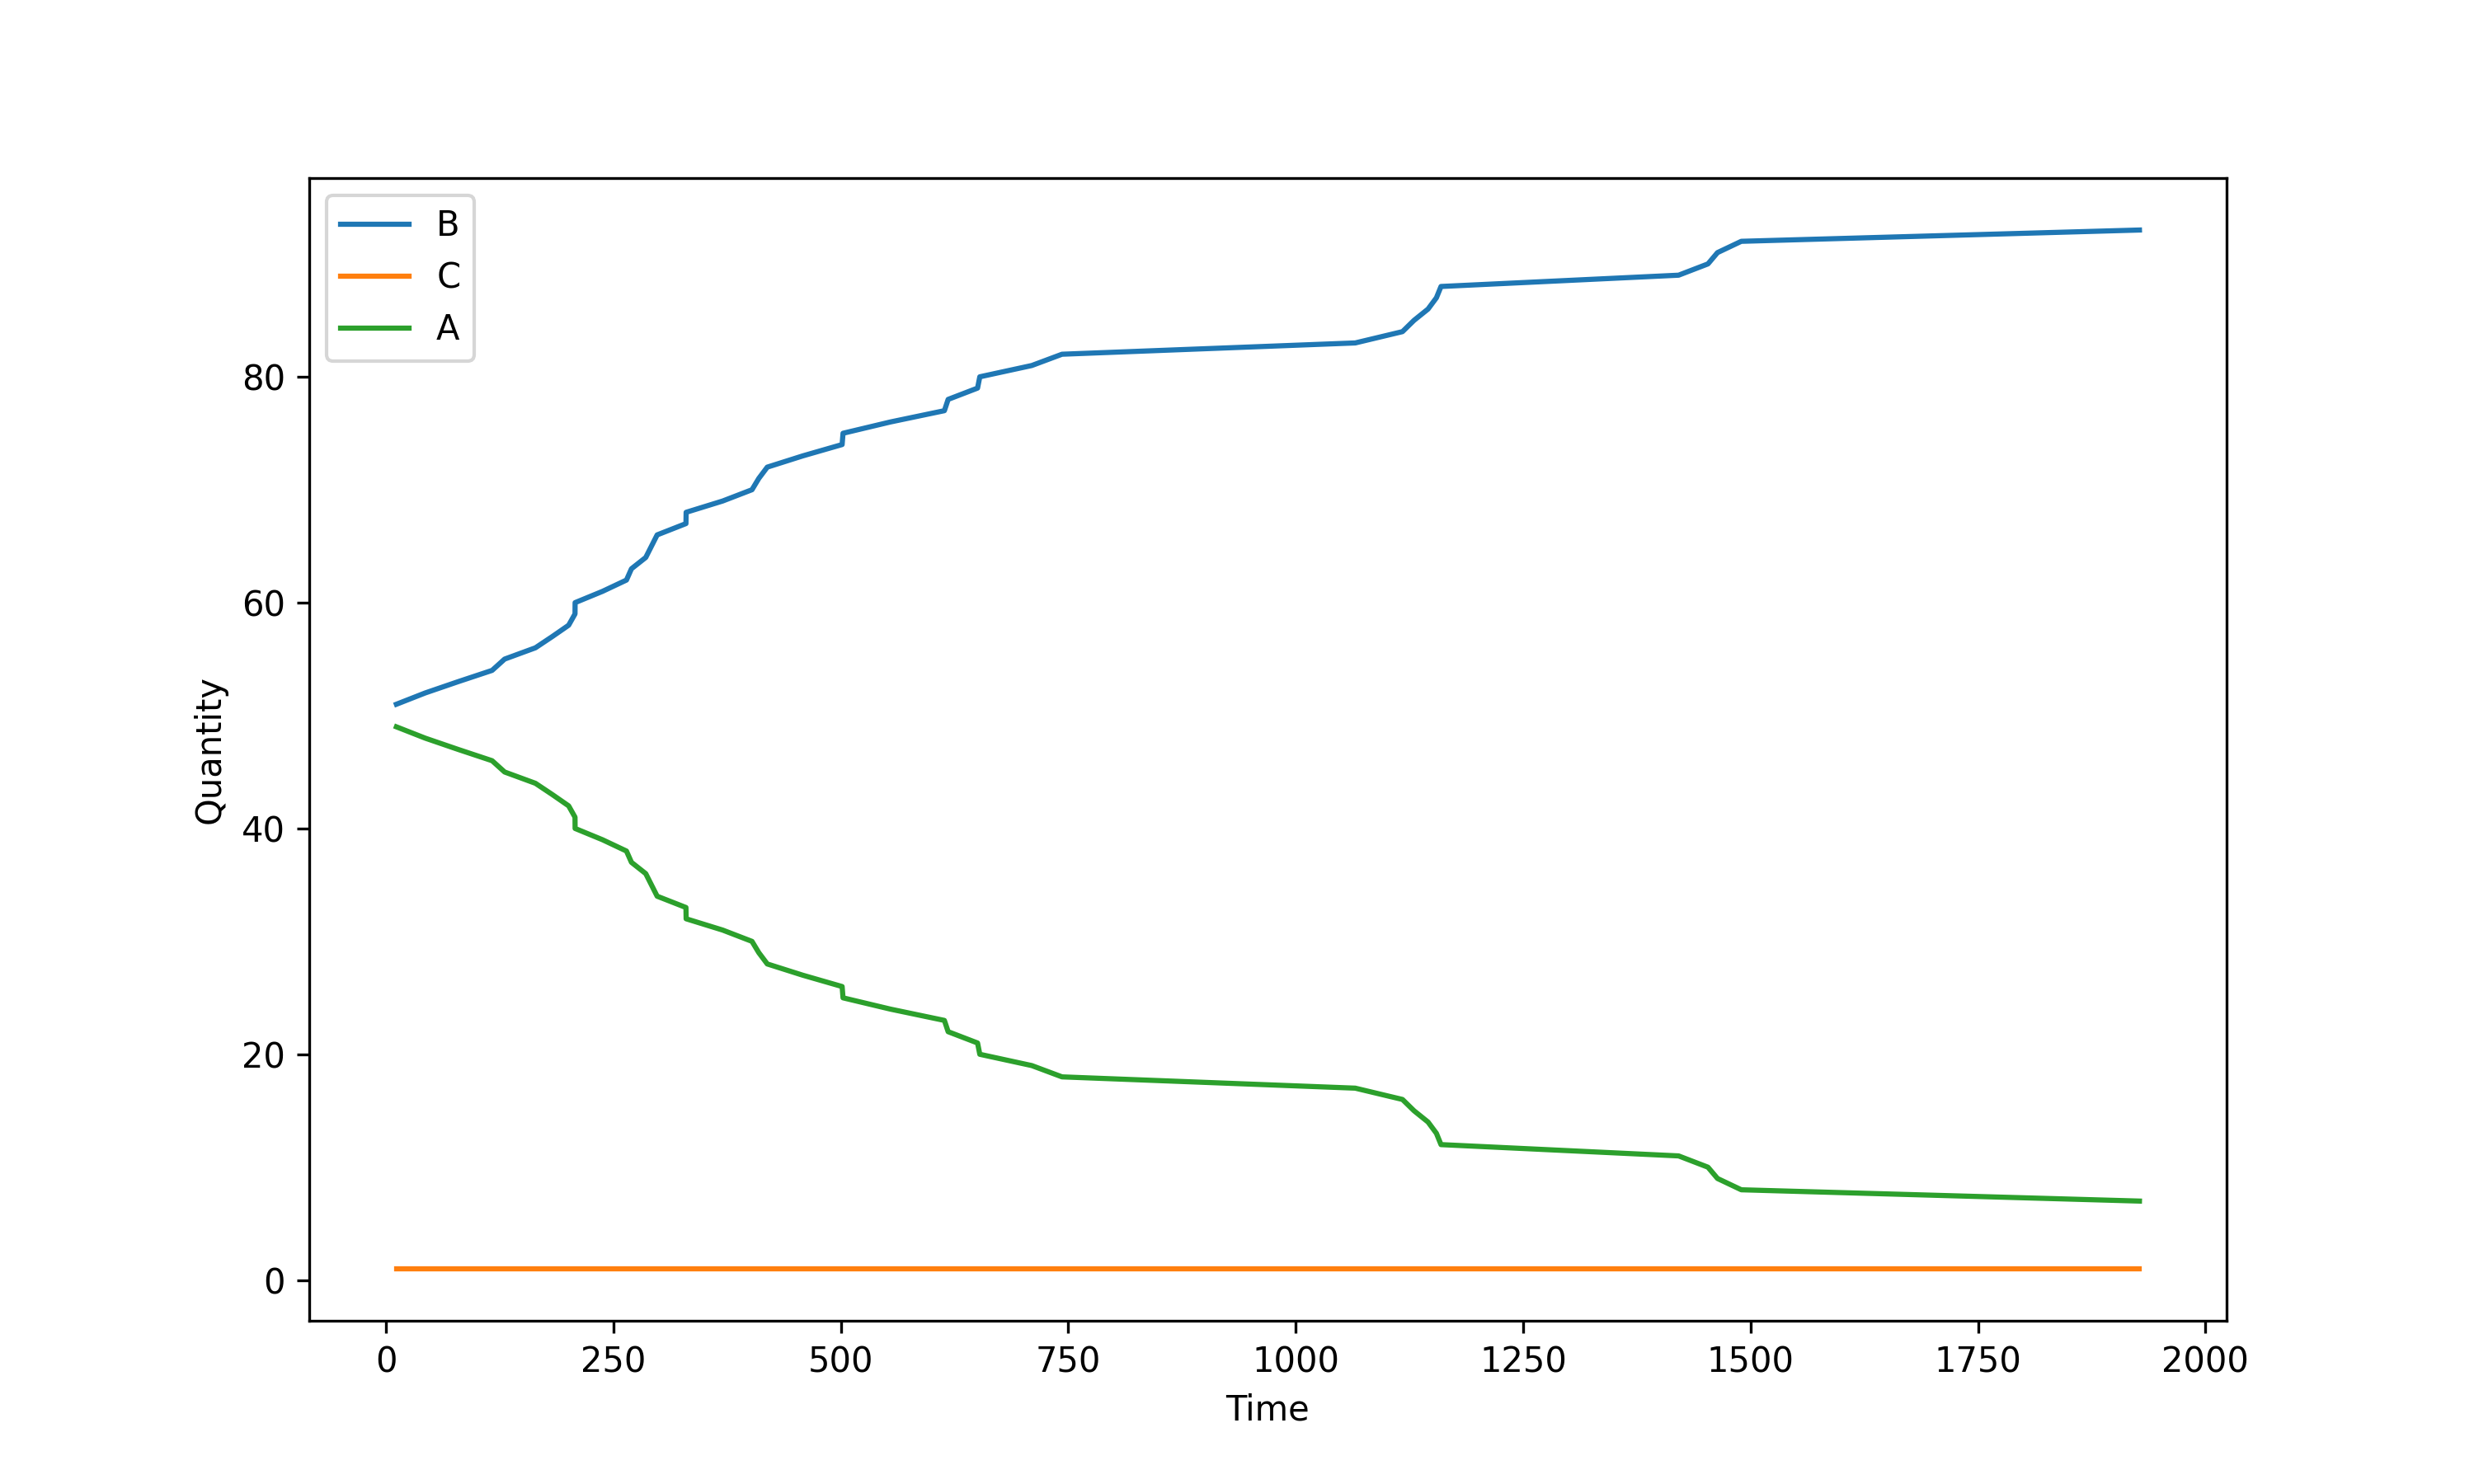
\includegraphics[width=\textwidth]{../plots/simple3}
	\caption{Plot of running the simple model simulation with A(0)=50, B(0)=50, C(0)=1.}
	\label{fig:plot_simple3}
\end{figure}

\begin{figure}[H]
	\centering
	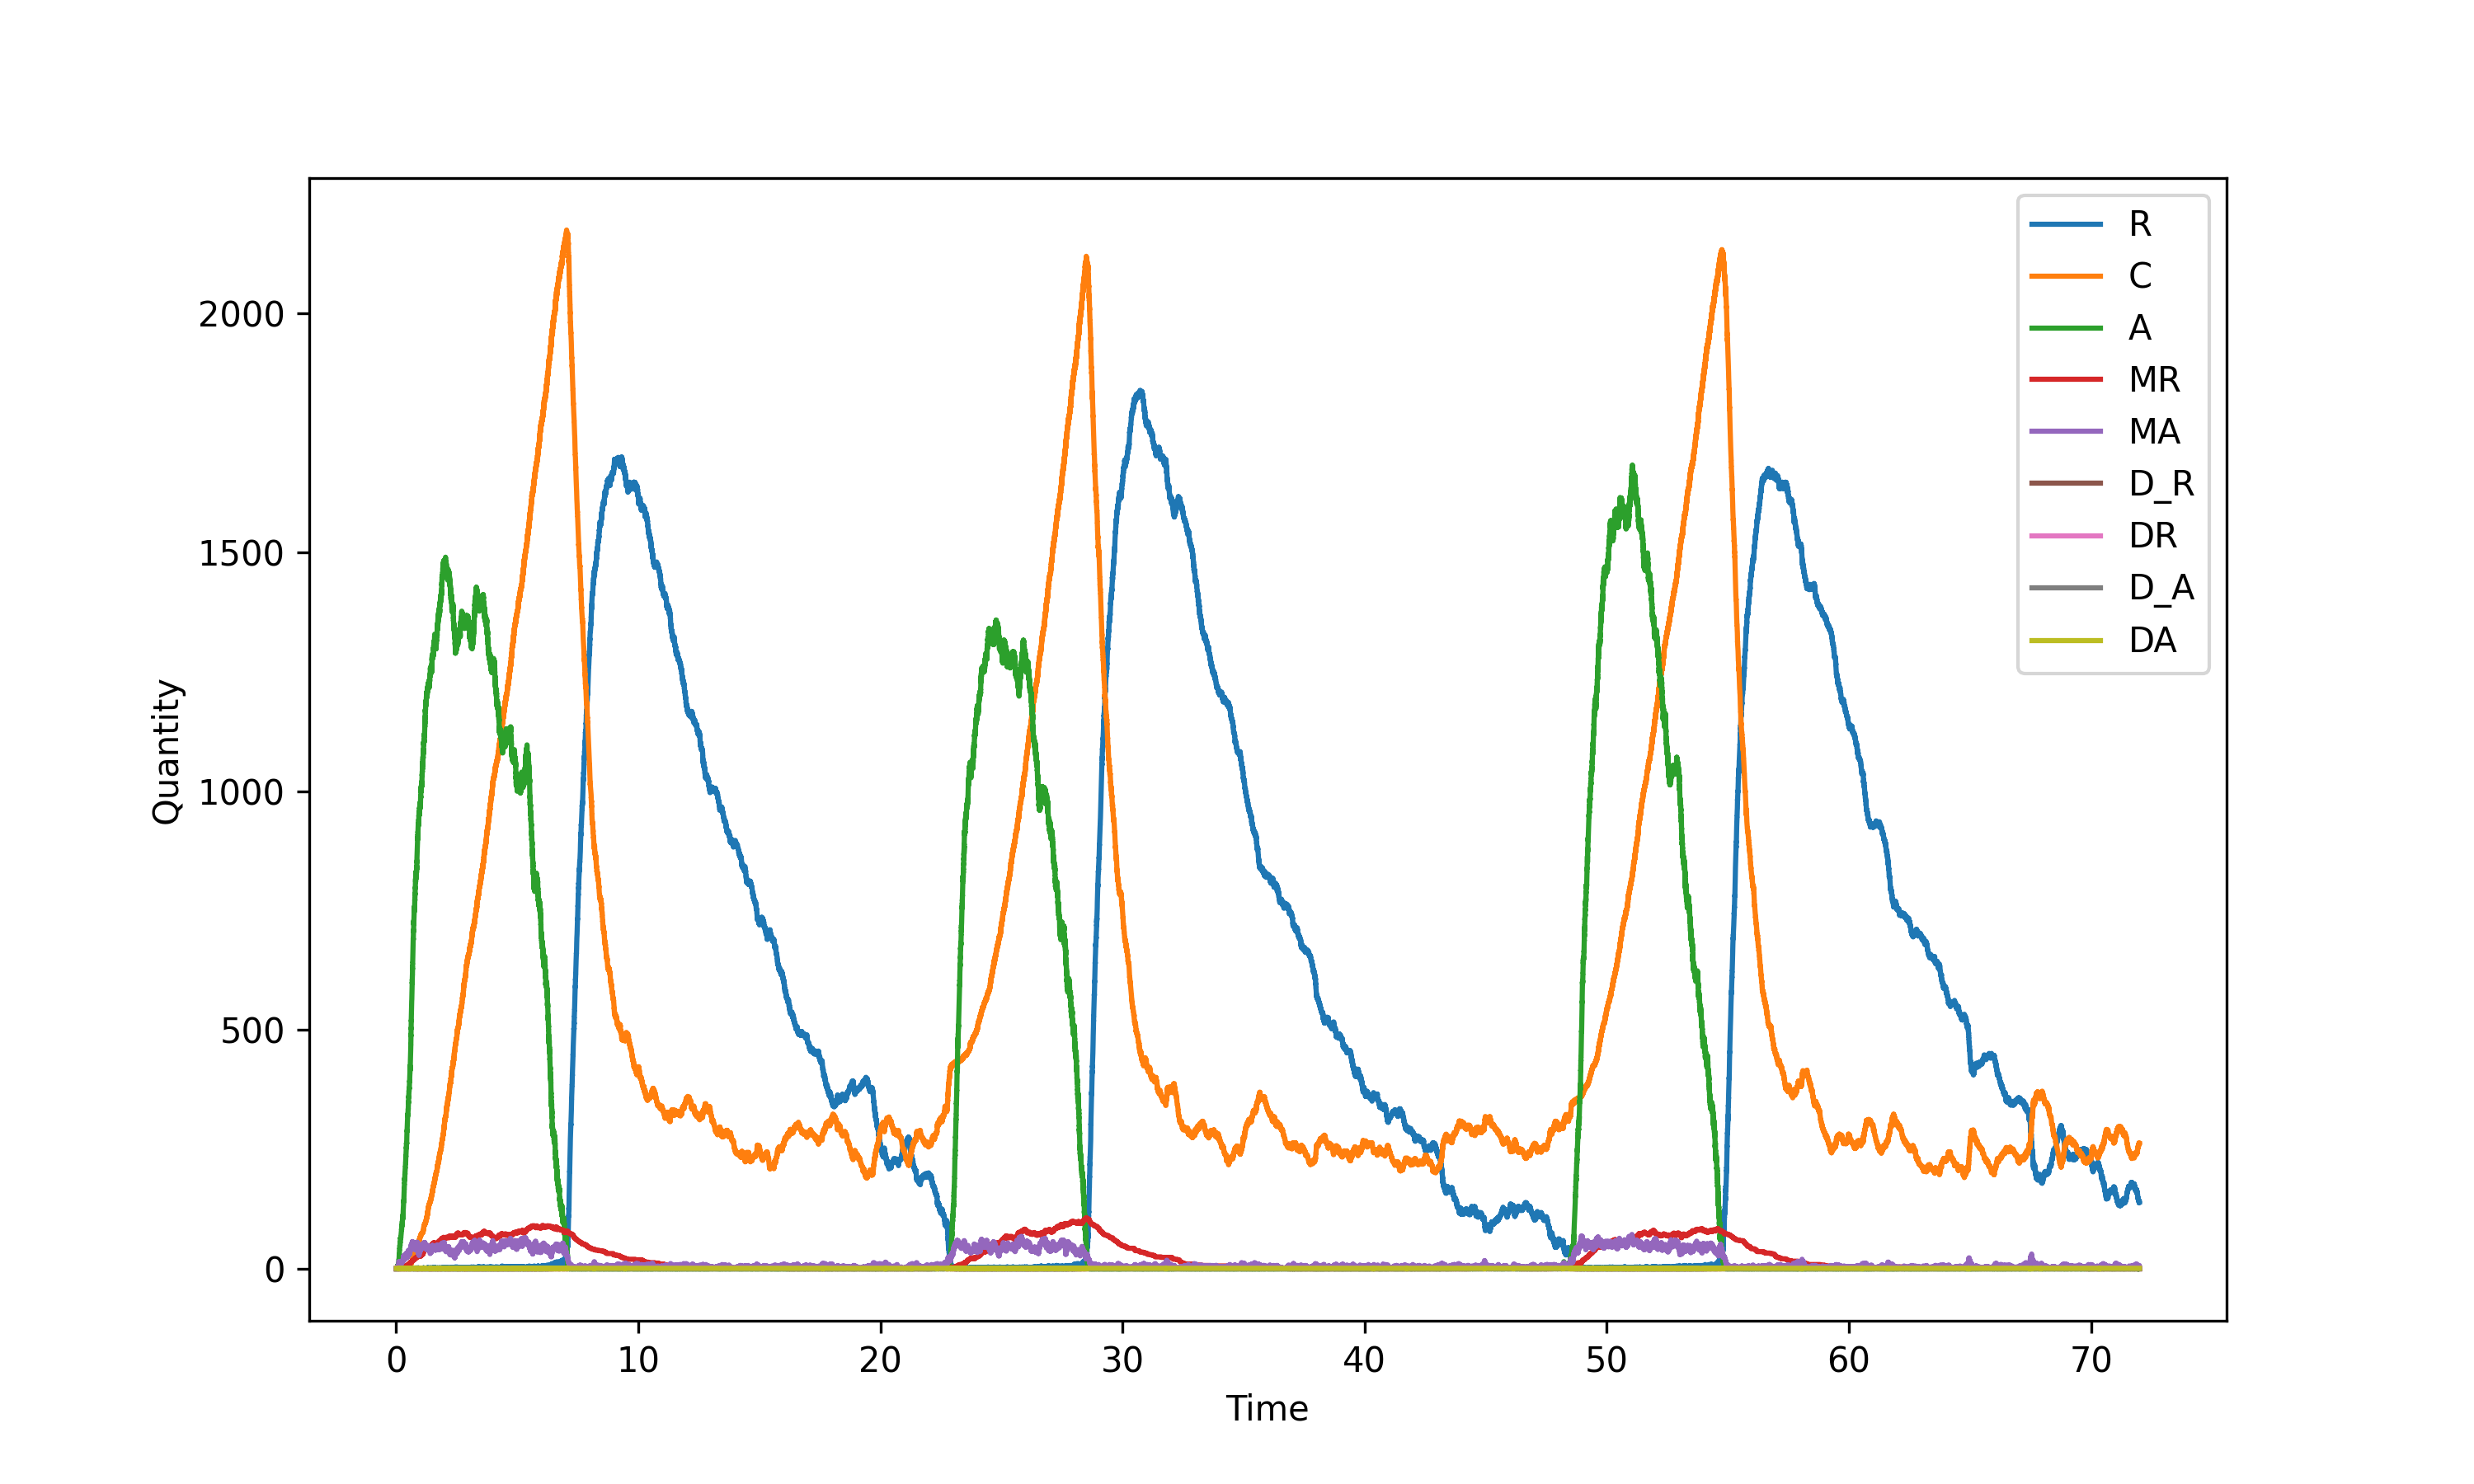
\includegraphics[width=\textwidth]{../plots/circadianOscillator.png}
	\caption{Plot of running the circadian oscillator model simulation.}
	\label{fig:plot_circadianOscillator}
\end{figure}

\begin{figure}[H]
	\centering
	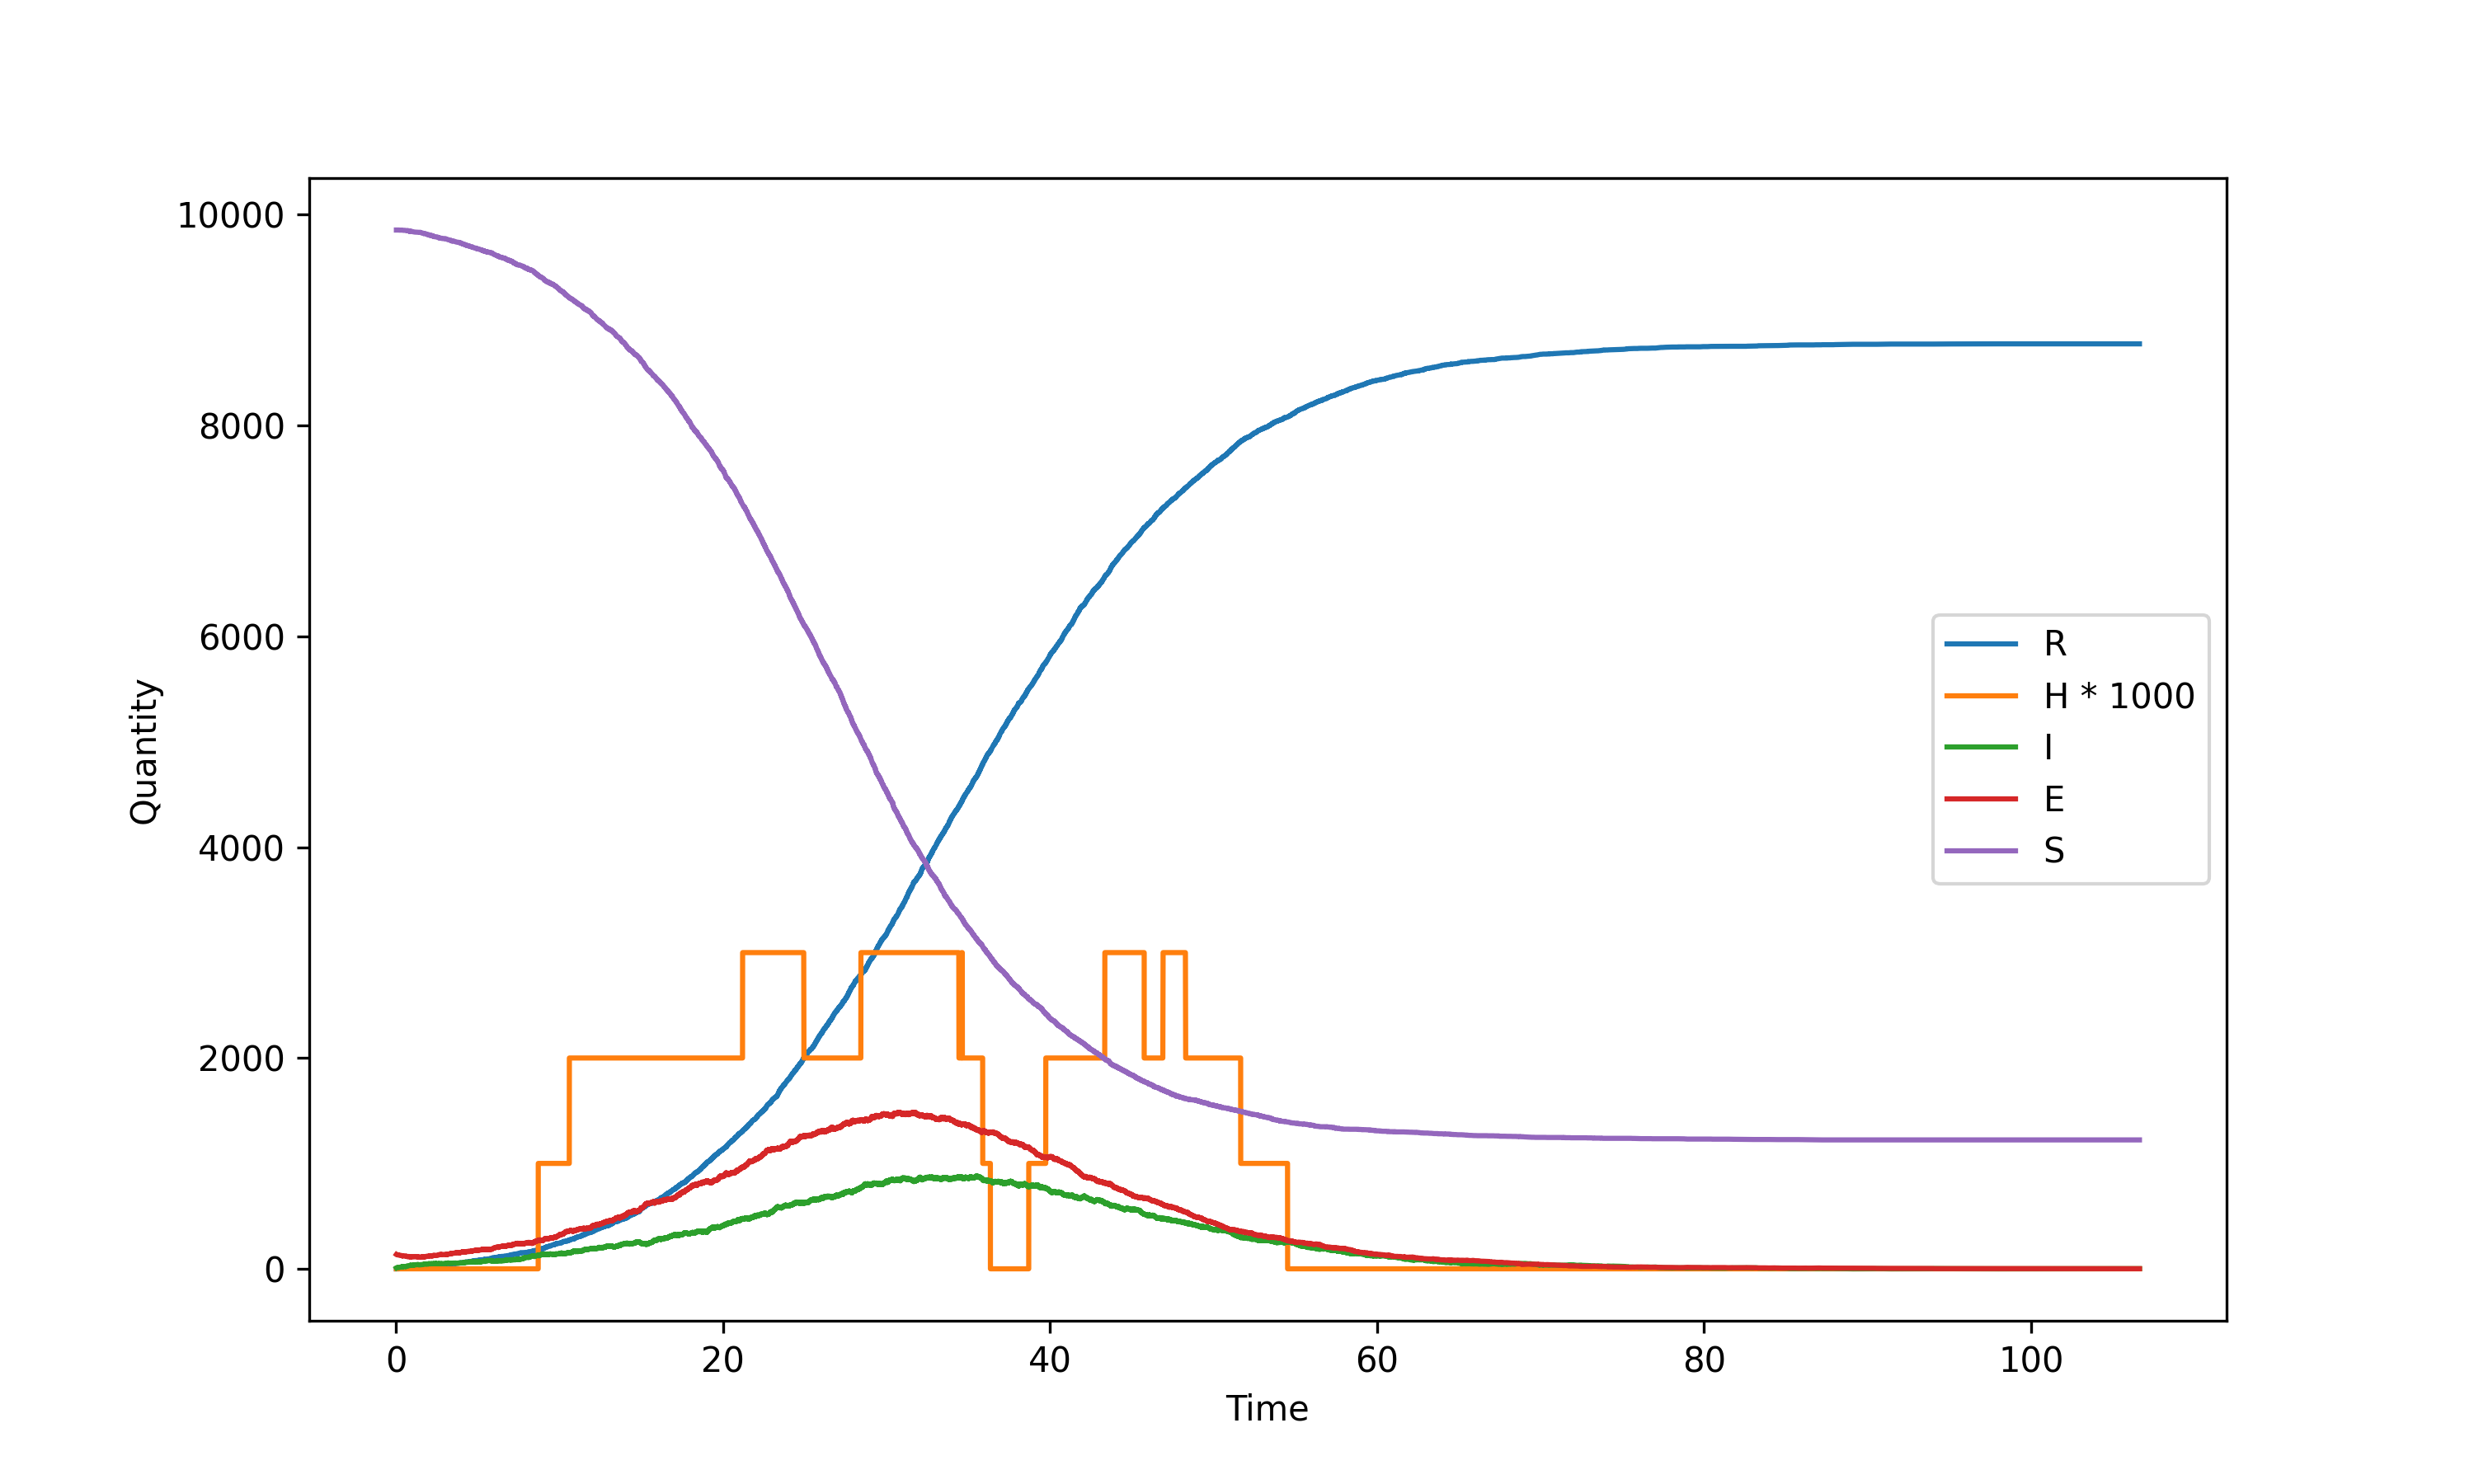
\includegraphics[width=\textwidth]{../plots/seihr.png}
	\caption{Plot of running the SEIHR model simulation.}
	\label{fig:plot_seihr}
\end{figure}

\subsection{Benchmarks}
\begin{figure}[H]
	\centering
	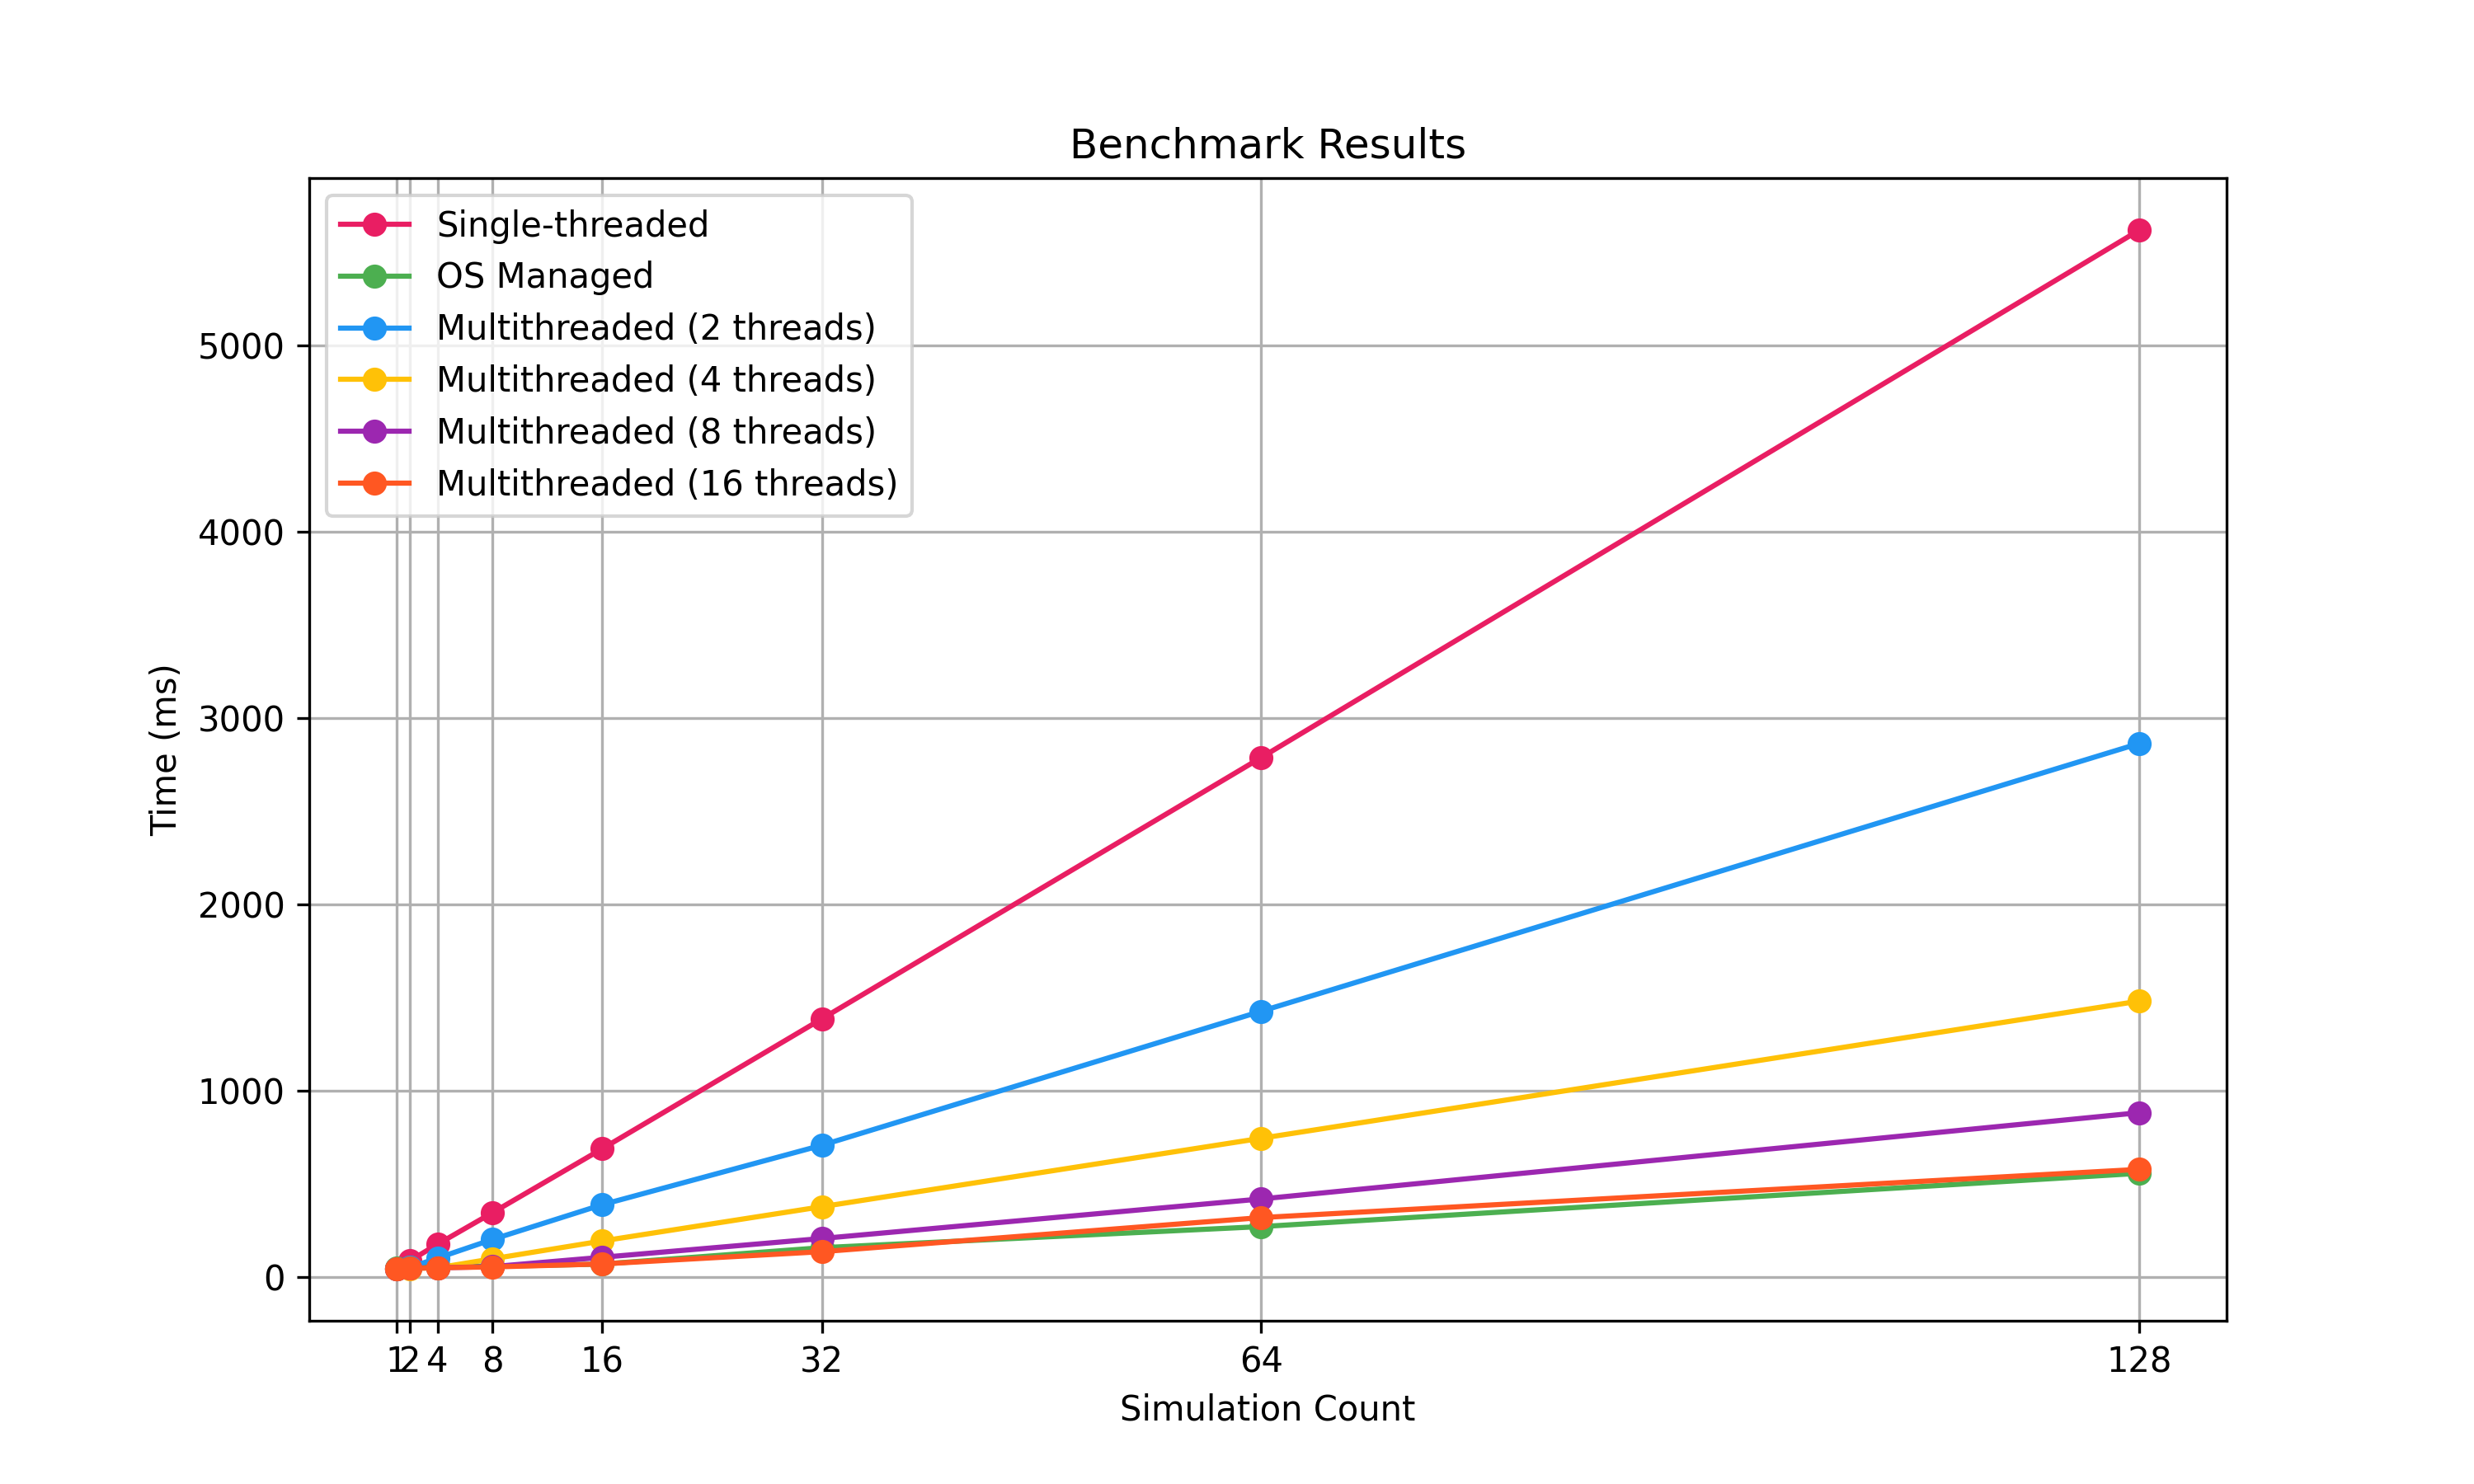
\includegraphics[width=\textwidth]{../benchmark/multithread_benchmark_with_sync.png}
	\caption{Benchmark of model simulation.}
	\label{fig:benchmark_multithread_with_sync}
\end{figure}

\begin{figure}[H]
	\centering
	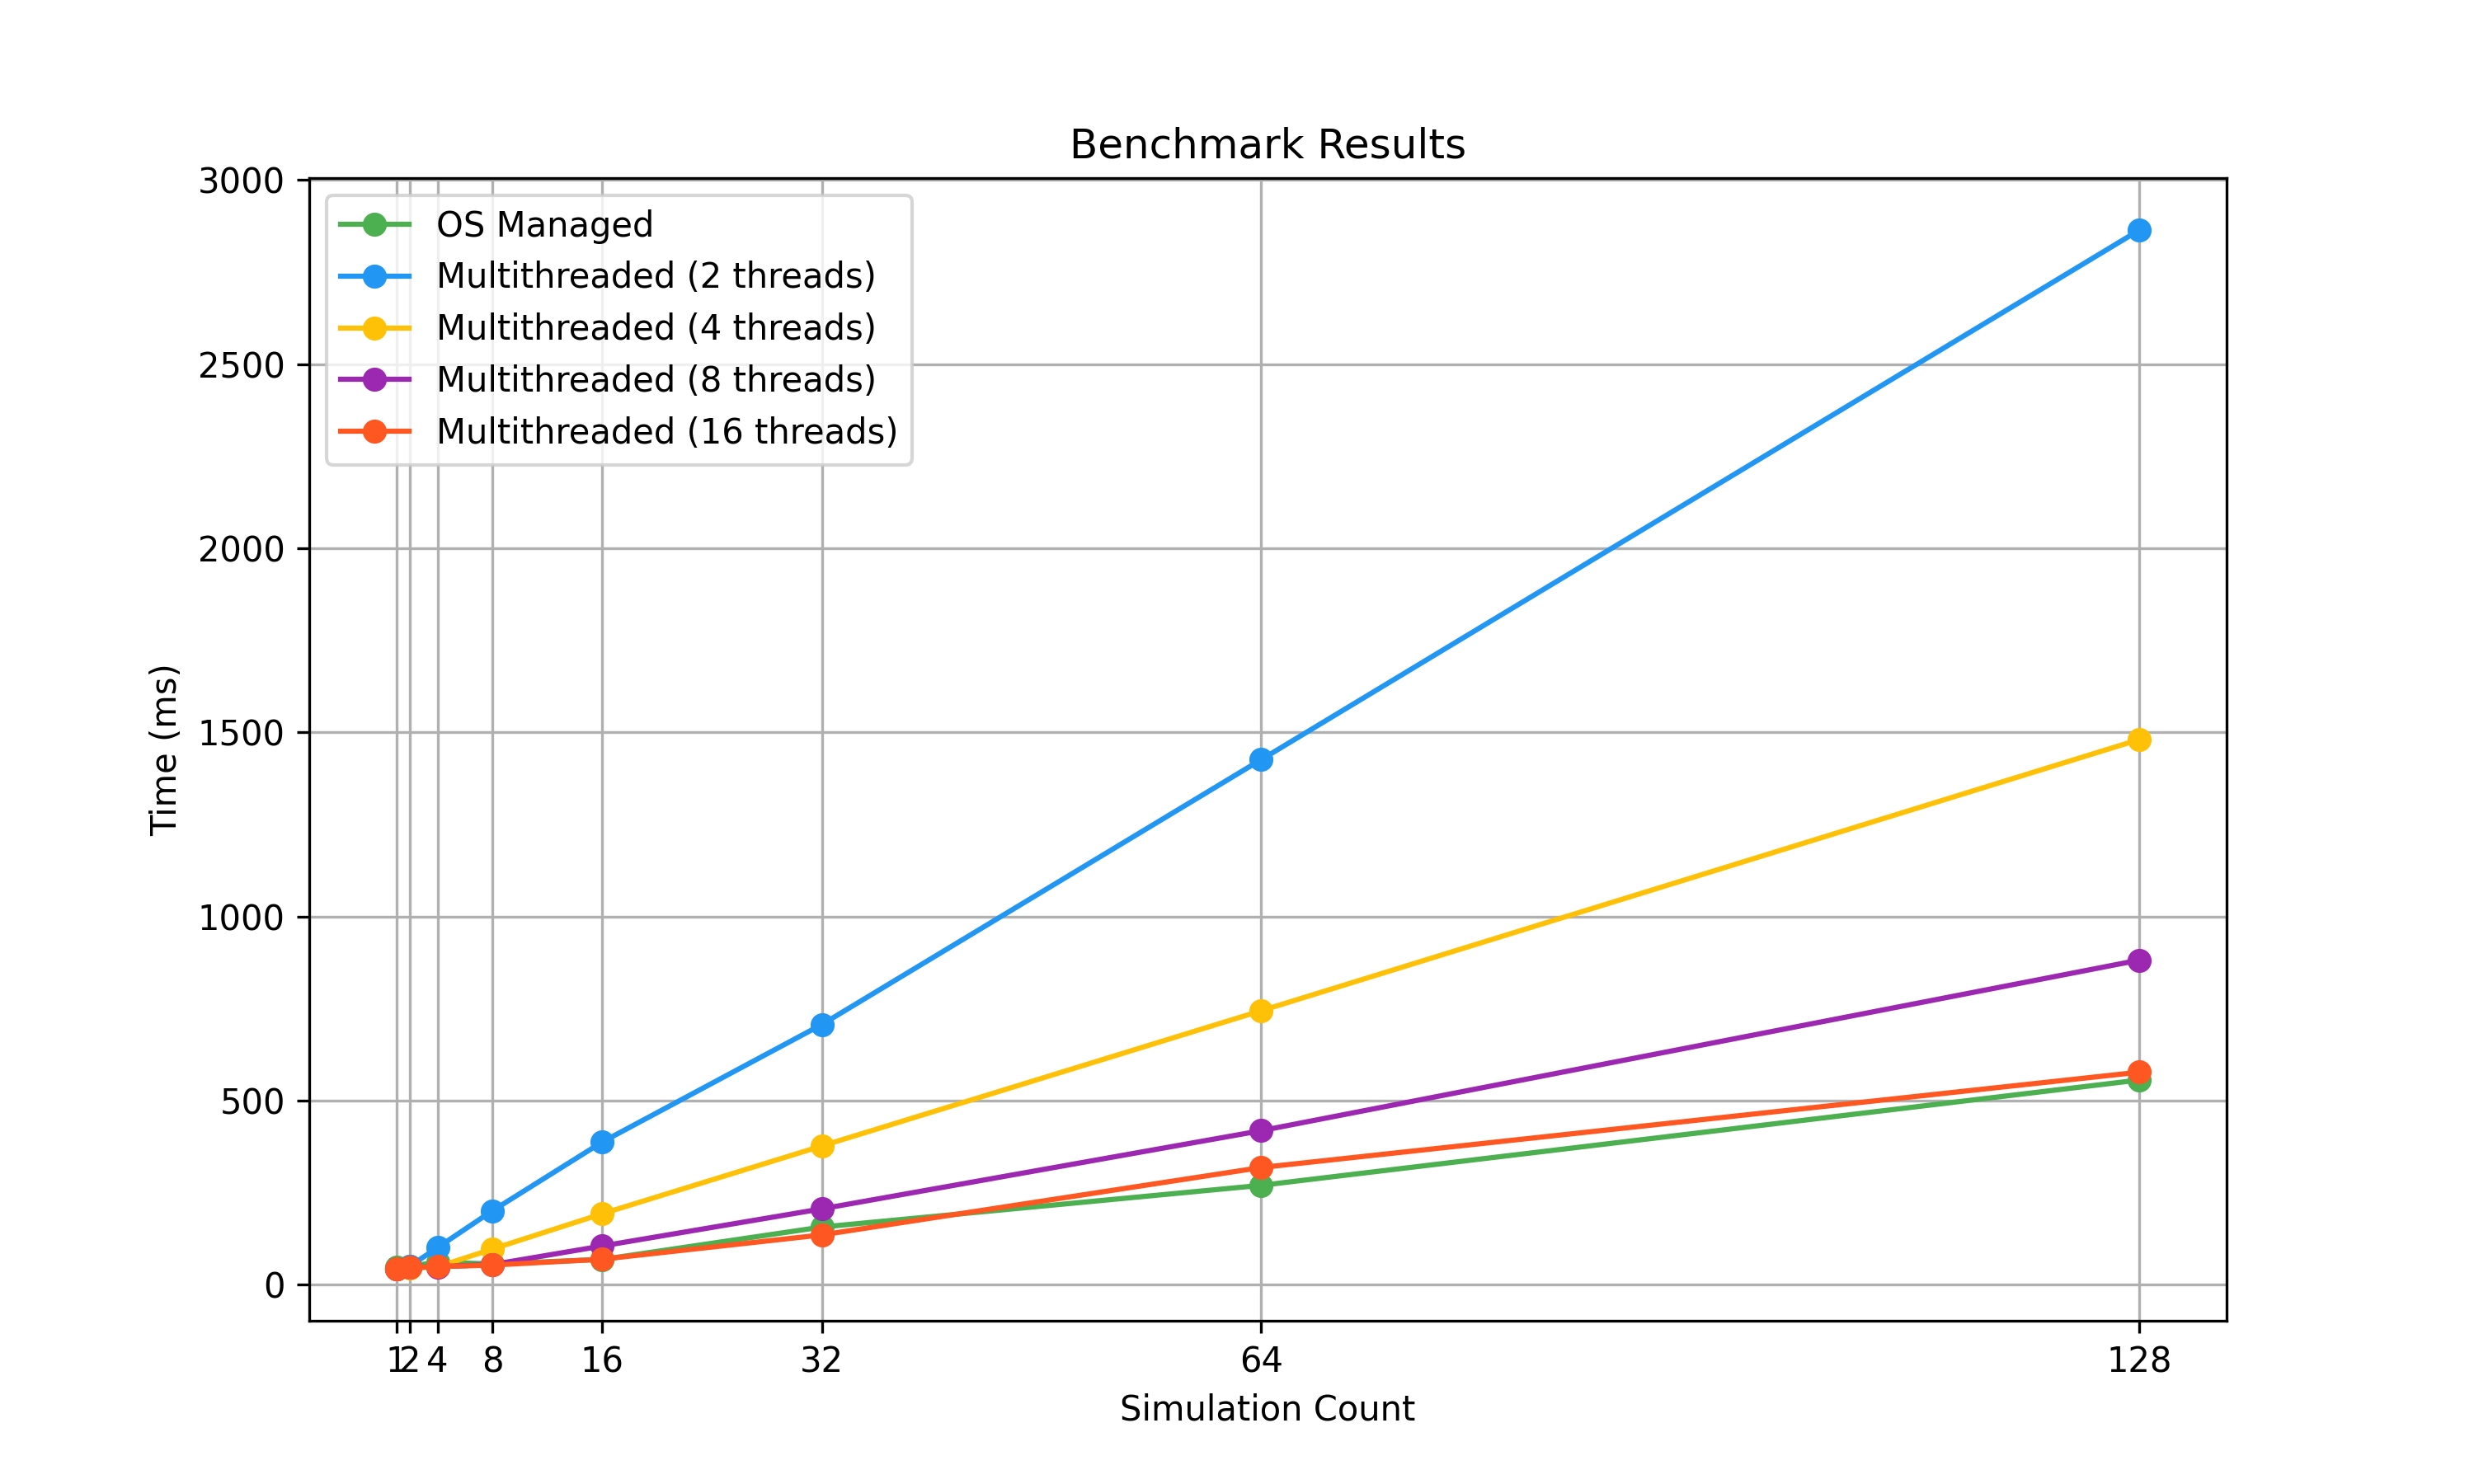
\includegraphics[width=\textwidth]{../benchmark/multithread_benchmark_without_sync.png}
	\caption{Benchmark of model simulation not including benchmarks for synchronized model simulation.}
	\label{fig:benchmark_multithread_without_sync}
\end{figure}

\section{Conclusions}
This section contains the results and conclusions of estimating the number of infected people in Denmark and North Jutland, as well as the benchmarks for running the simulations in parallel and sequentially.

\subsection{Estimations}
The following table shows the estimations for the number of infected people in Denmark (DK) as well as North Jutland (NJ) specifically.
These estimations were calculated by running the \texttt{main} function in Listing \ref{lst:EstimationsMain.cpp}.

\begin{table}[h]
\centering
\begin{tabular}{|c|c|c|}
\hline
& \textbf{Mean Hospitalized} & \textbf{Peak Hospitalized} \\
\hline
DK & 1193 & 1268 \\
NJ & 128 & 161 \\
\hline
\end{tabular}
\caption{Hospitalization estimations.}
\label{tab:hospitalization_estimations}
\end{table}

\subsection{Benchmarks}
The benchmarks clearly indicate that running multiple simulations in parallel is faster than running them sequentially.
This is to be expected, as the simulations are independent of each other, and can therefore be run in parallel without any issues.
In other words, there are no data dependencies between the simulations, and therefore no need to wait for one simulation to finish before starting the next one.

As is also expected, running the simulations on a 16 core machine and letting the OS schedule the threads is about the same as running the simulations in a thread pool with 16 threads.
According to my results, at least, the difference is negligible.


\end{document}
